\chapter{代数的集合とZariski位相}
\label{ch:ch03}

\begin{chapterlead}
本章では，代数幾何学の舞台となる「アフィン空間」と，その中で多項式の共通零点として定まる図形「代数的集合」を導入する．
代数的集合全体は和集合と共通部分について閉じており，これを閉集合系とする位相が \textbf{Zariski位相} である．
Zariski位相は通常の（Euclid的な）位相に比べて極端に粗く，Hausdorffでさえないが，多項式という「硬い」関数だけで幾何学を語るための自然な言語である．
後半では，図形を「これ以上分解できない部分」に分ける \textbf{既約分解} を扱い，Noether性（第2章）から既約分解の存在と一意性が従うことを示す．
既約性が座標環の整域性，すなわち消滅イデアルの素性と同値であることも述べるが，イデアルと図形の対応の全体像は第4章で Hilbert の零点定理とともに完成する．
\end{chapterlead}

本章を通して $k$ は体とし，特に断らない限り代数閉体（典型的には $k=\C$）とする．
ただし本章の議論の大半は $k$ が無限体でありさえすれば成り立つ．
$k$ が代数閉であることが本質的に効いてくるのは第4章の零点定理である．

%======================================================================
\section{アフィン空間}
%======================================================================

\subsection{アフィン空間の定義}

\begin{mydef}{アフィン空間}{ch03-affine-space}
体 $k$ と自然数 $n$ に対し，集合
\[
  \A^n = \A^n_k := \{(a_1,\dots,a_n) \mid a_i\in k\}
\]
を $k$ 上の \textbf{$n$次元アフィン空間} (affine $n$-space) とよぶ．
$\A^1$ を \textbf{アフィン直線}，$\A^2$ を \textbf{アフィン平面} という．
\end{mydef}

集合としては $\A^n$ は $k^n$ と全く同じである．
それでもわざわざ別の記号を用いるのは，$k^n$ が持っている \emph{ベクトル空間としての構造}（原点という特別な点，和とスカラー倍）を忘れ，
「点の集まり」として見ていることを強調するためである．
たとえば $\A^2$ の中の直線 $x+y=1$ は原点を通らないが，アフィン空間の立場からは原点を通る直線 $x+y=0$ と何ら区別すべき理由はない．
アフィン空間にはもう一つ，後で導入する Zariski 位相（\ref{sec:ch03-zariski}節）が入る．
したがって $\A^n$ は「$k^n$ という集合 $+$ Zariski 位相 $+$ 多項式関数の環」という三つ組として理解するのが正しい．

物理で言えば，Minkowski 時空は「原点を持たない」アフィン空間であり，二点の差（変位ベクトル）だけが意味を持つ．
代数幾何学における $\A^n$ もこれと同じ精神で導入される．

\begin{myex}{低次元のアフィン空間}{ch03-low-dim}
\begin{itemize}
  \item $\A^0$ は一点からなる集合である．
  \item $k=\R$ のとき $\A^1_\R$ は実数直線，$\A^2_\R$ は実平面であり，絵に描くことができる．
  \item $k=\C$ のとき $\A^1_\C=\C$ は実2次元の複素平面であり，$\A^2_\C=\C^2$ は実4次元である．
        したがって複素代数曲線（$\A^2_\C$ 内の1次元の図形）は実2次元の曲面であり，絵を描くときは実部だけを描いて代用することが多い．
\end{itemize}
\end{myex}

\subsection{座標表示}

$\A^n$ の点 $P$ は $n$ 個の数の組 $P=(a_1,\dots,a_n)$ で与えられ，$a_i$ を $P$ の \textbf{座標} という．
座標を読み取る写像
\[
  x_i \colon \A^n \to k,\qquad (a_1,\dots,a_n)\mapsto a_i
\]
を \textbf{座標関数} とよぶ．代数幾何学では，$x_i$ を「変数」というよりも「$\A^n$ 上の関数」として見る観点が重要である．
多項式環 $k[x_1,\dots,x_n]$ の不定元 $x_i$ と座標関数 $x_i$ を同じ記号で書くのは，この二つを同一視するためである．

座標は一意ではない．可逆な \textbf{アフィン変換}
\[
  \bm{x} \longmapsto A\bm{x}+\bm{b},\qquad A\in\GL_n(k),\ \bm{b}\in k^n
\]
によって新しい座標系に移ることができ，アフィン空間の幾何学的な性質はこのような座標変換で変わらないものとして定式化される．
後に見るように，代数幾何学で許される座標変換はさらに広く，多項式で書けて逆も多項式で書ける写像（多項式自己同型）全体である．
たとえば $\A^2$ において
\[
  (x,y)\longmapsto (x,\ y+x^2)
\]
は逆写像 $(x,y)\mapsto (x,\,y-x^2)$ を持つので座標変換とみなせる．
これにより放物線 $y=x^2$ は直線 $y=0$ に写る（図\ref{fig:ch03-parabola-straighten}）．
アフィン変換では放物線を直線に写すことはできないから，代数幾何学の「座標変換」は線形代数のそれよりもずっと柔軟である．

\begin{figure}[H]
\centering
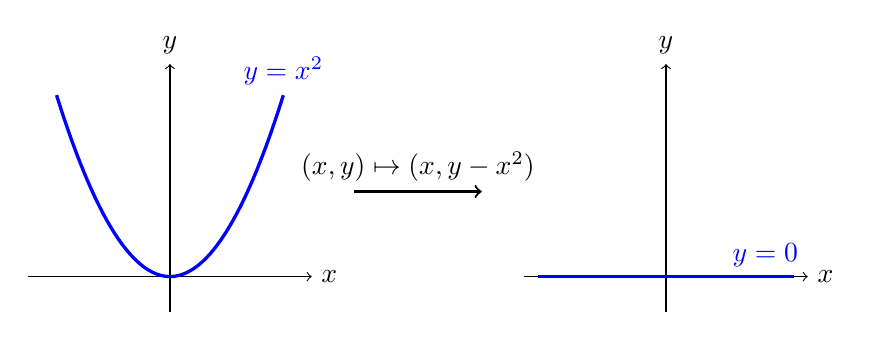
\begin{tikzpicture}[scale=0.9]
  \begin{scope}
    \draw[->] (-2,0)--(2,0) node[right]{$x$};
    \draw[->] (0,-0.5)--(0,3) node[above]{$y$};
    \draw[very thick,blue,domain=-1.6:1.6,samples=60] plot (\x,{\x*\x});
    \node[blue] at (1.6,2.9) {$y=x^2$};
  \end{scope}
  \draw[->,thick] (2.6,1.2)--(4.4,1.2) node[midway,above]{$(x,y)\mapsto(x,y-x^2)$};
  \begin{scope}[xshift=7cm]
    \draw[->] (-2,0)--(2,0) node[right]{$x$};
    \draw[->] (0,-0.5)--(0,3) node[above]{$y$};
    \draw[very thick,blue] (-1.8,0)--(1.8,0);
    \node[blue,above] at (1.4,0) {$y=0$};
  \end{scope}
\end{tikzpicture}
\caption{多項式自己同型による放物線の「まっすぐ化」．}
\label{fig:ch03-parabola-straighten}
\end{figure}

\subsection{アフィン空間上の多項式関数}

多項式 $f\in k[x_1,\dots,x_n]$ は，各点で値を代入することにより関数
\[
  f\colon \A^n\to k,\qquad P=(a_1,\dots,a_n)\mapsto f(P)=f(a_1,\dots,a_n)
\]
を定める．このような関数を \textbf{多項式関数} (polynomial function) あるいは \textbf{正則関数} という．
多項式関数どうしの和・積はまた多項式関数であり，多項式関数全体は $k$ 上の可換環をなす．
この環が多項式環そのものと一致するかどうかは自明ではない．

\begin{myprop}{多項式と多項式関数}{ch03-poly-function}
$k$ が無限体ならば，写像
\[
  k[x_1,\dots,x_n]\longrightarrow \{\A^n\text{ 上の関数}\},\qquad f\mapsto (P\mapsto f(P))
\]
は単射である．すなわち，$\A^n$ の全ての点で値が $0$ になる多項式は零多項式に限る．
\end{myprop}

\begin{proof}
第1章の命題\ref{prop:ch01-poly-function}と同じ主張である（一変数の場合に根の個数が次数以下であることを用い，変数の個数に関する帰納法で示す）．
\end{proof}

有限体ではこの命題は成り立たない．たとえば $k=\F_p$ 上で $f=x^p-x$ は零多項式ではないが，Fermat の小定理により全ての点で $0$ になる．
これが，代数幾何学の素朴な理論を無限体（とくに代数閉体）上で展開する理由の一つである．
有限体上の幾何学をきちんと扱うには，第12章のスキーム論の言葉が必要になる．

\subsection{アフィン空間の幾何学的構造}

$\A^n$ の上に定義される「幾何学的構造」とは何だろうか．微分幾何学では，多様体の構造はその上の滑らかな関数のなす環で決まる．
同様に代数幾何学では，$\A^n$ の構造は
\[
  \text{多項式関数の環}\quad k[\A^n] := k[x_1,\dots,x_n]
\]
によって規定されると考える．距離や角度，あるいは「近さ」といった概念は，あらかじめ与えるものではなく，多項式関数から引き出されるべきものである．
たとえば「点 $P$ の近く」という概念は，「$P$ で $0$ にならない多項式 $f$ について，$f\ne 0$ となる点の集合」という形で定式化される（\ref{sec:ch03-zariski}節の基本開集合）．
また $\A^n$ の部分集合のうちで「意味のある図形」とは，多項式で記述できるもの，すなわち次節以降で扱う零点集合である．

まとめると，本書における基本的な視点は次の対応である：
\begin{center}
\begin{tabular}{c|c}
幾何学 & 代数学 \\ \hline
アフィン空間 $\A^n$ & 多項式環 $k[x_1,\dots,x_n]$ \\
点 $P\in\A^n$ & 値を代入する操作 $f\mapsto f(P)$ \\
図形（代数的集合） & 多項式の集合（イデアル）
\end{tabular}
\end{center}
この対応を精密にすることが本章と第4章の目標である．

\begin{physbox}[配位空間と場の空間]
物理において，$N$ 個のスカラー場 $\phi_1,\dots,\phi_N$ の値の空間（場の空間，target space）は典型的には $\C^N$ であり，
ポテンシャルや超ポテンシャルは $\phi_i$ の多項式で与えられることが多い．
このとき場の空間を「アフィン空間 $\A^N_\C$」として見るのは自然である．
場の再定義 $\phi\mapsto \phi'$ のうち多項式で書けて逆も多項式で書けるものは，ラグランジアンの多項式性を保つ「許される場の再定義」であり，
上で述べた多項式自己同型はちょうどこれに相当する．
\end{physbox}

\exprob{prob:ch03-1} $k=\F_2$ とする．$\A^2_{\F_2}$ の4点すべてで値が $0$ になる零でない多項式 $f\in\F_2[x,y]$ を一つ挙げよ．また，このような $f$ 全体がイデアル $(x^2-x,\ y^2-y)$ と一致することを示せ．

\exprob{prob:ch03-2} 写像 $\varphi\colon\A^2\to\A^2$, $(x,y)\mapsto(x+y^3,\ y)$ が多項式自己同型であることを示し，逆写像を求めよ．また $\varphi$ による曲線 $x=0$ の像を求めよ．

%======================================================================
\section{多項式集合の零点}
%======================================================================

\subsection{多項式集合 $S$ に対する零点集合}

\begin{mydef}{零点集合}{ch03-zero-set}
$S\subset k[x_1,\dots,x_n]$ を多項式の集合とする．
\[
  \Zero(S) := \{P\in\A^n \mid \text{すべての } f\in S \text{ に対し } f(P)=0\}
\]
を $S$ の \textbf{零点集合} (zero locus, vanishing set) という．
$S=\{f_1,\dots,f_r\}$ が有限集合のときは $\Zero(f_1,\dots,f_r)$ と書く．
\end{mydef}

$\Zero(S)$ は「$S$ に属する多項式方程式の連立方程式の解集合」にほかならない．
$S$ は無限集合でも構わないが，後で見るように（命題\ref{prop:ch03-finite-gen}），実は常に有限個の多項式で置き換えられる．

\subsection{単一の多項式が定める集合}

$f$ を定数でない多項式とするとき，$\Zero(f)$ を \textbf{超曲面} (hypersurface) という．
$n=2$ のときは \textbf{平面曲線}，$n=3$ のときは（狭い意味の）\textbf{曲面} である．

\begin{myex}{平面曲線}{ch03-plane-curves}
$\A^2_\R$ の中で次の零点集合を考える（図\ref{fig:ch03-curves}）．
\begin{enumerate}
  \item $\Zero(x^2+y^2-1)$：単位円．
  \item $\Zero(y^2-x^3)$：原点に尖点 (cusp) を持つ曲線．
  \item $\Zero(y^2-x^2(x+1))$：原点で自分自身と交わる曲線（結節点，node）．
  \item $\Zero(xy)$：二本の座標軸の和集合．
\end{enumerate}
$f$ が一つでも，$\Zero(f)$ は滑らかとは限らず（2, 3），いくつかの部分の和集合になることもある（4）．
これらの現象は第7章（特異点）と本章\ref{sec:ch03-irred}節（既約性）でそれぞれ扱う．
\end{myex}

\begin{figure}[H]
\centering
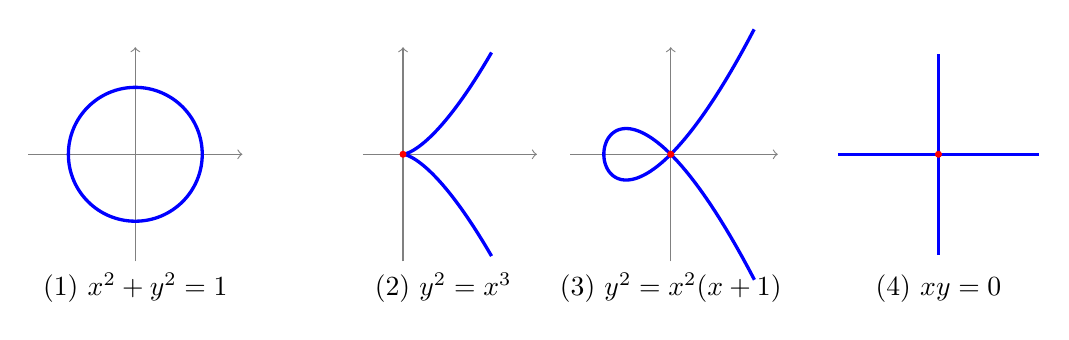
\begin{tikzpicture}[scale=0.85]
  % circle
  \begin{scope}
    \draw[->,gray] (-1.6,0)--(1.6,0); \draw[->,gray] (0,-1.6)--(0,1.6);
    \draw[very thick,blue] (0,0) circle (1);
    \node at (0,-2.0) {(1) $x^2+y^2=1$};
  \end{scope}
  % cusp
  \begin{scope}[xshift=4cm]
    \draw[->,gray] (-0.6,0)--(2,0); \draw[->,gray] (0,-1.6)--(0,1.6);
    \draw[very thick,blue,domain=-1.15:1.15,samples=80] plot ({\x*\x},{\x*\x*\x});
    \fill[red] (0,0) circle (1.5pt);
    \node at (0.6,-2.0) {(2) $y^2=x^3$};
  \end{scope}
  % node
  \begin{scope}[xshift=8cm]
    \draw[->,gray] (-1.5,0)--(1.6,0); \draw[->,gray] (0,-1.6)--(0,1.6);
    \draw[very thick,blue,domain=-1.5:1.5,samples=100] plot ({\x*\x-1},{\x*(\x*\x-1)});
    \fill[red] (0,0) circle (1.5pt);
    \node at (0,-2.0) {(3) $y^2=x^2(x+1)$};
  \end{scope}
  % xy=0
  \begin{scope}[xshift=12cm]
    \draw[very thick,blue] (-1.5,0)--(1.5,0);
    \draw[very thick,blue] (0,-1.5)--(0,1.5);
    \fill[red] (0,0) circle (1.5pt);
    \node at (0,-2.0) {(4) $xy=0$};
  \end{scope}
\end{tikzpicture}
\caption{一つの多項式で定まる平面曲線（実部）．赤い点は特異点．}
\label{fig:ch03-curves}
\end{figure}

\paragraph{超曲面の次元についての直感．}
$\A^n$ の中で方程式を一本課すと自由度が一つ減るので，$\Zero(f)$ は $(n-1)$ 次元の図形になると期待される．
$k$ が代数閉体であれば，定数でない $f$ に対して $\Zero(f)$ は空でなく（一変数ならば代数学の基本定理そのもの），実際 $(n-1)$ 次元になる（次元の厳密な定義と証明は第7章）．
一方 $k=\R$ では $\Zero(x^2+y^2+1)=\emptyset$ や $\Zero(x^2+y^2)=\{(0,0)\}$ のように，次元の直感が破れる．
これが複素数上で考える大きな理由である（第1章参照）．

\subsection{複数の多項式が定める集合}

複数の多項式 $f_1,\dots,f_r$ に対して，定義から直ちに
\[
  \Zero(f_1,\dots,f_r) = \Zero(f_1)\cap\cdots\cap\Zero(f_r)
\]
である．すなわち連立方程式の解集合は各超曲面の共通部分である．

\begin{myex}{空間曲線}{ch03-space-curve}
$\A^3$ において，
\[
  C = \Zero(y-x^2,\ z-x^3)
\]
は二つの曲面 $y=x^2$（放物柱面）と $z=x^3$ の交わりであり，$t\mapsto (t,t^2,t^3)$ と媒介変数表示される曲線である．
これを \textbf{ねじれ3次曲線} (twisted cubic) という．方程式は2本，次元は $3-2=1$ である．
\end{myex}

\begin{myex}{方程式の数と次元が合わない例}{ch03-not-ci}
$\A^3$ において
\[
  X = \Zero(xz,\ yz)
\]
を考える．$xz=yz=0$ は「$z=0$ または $x=y=0$」と同値なので，
$X$ は平面 $\{z=0\}$ と直線 $\{x=y=0\}$（$z$ 軸）の和集合である（図\ref{fig:ch03-plane-line}）．
方程式は2本だが，$X$ には2次元の部分と1次元の部分が混在している．
「方程式の数 $=$ 余次元」という素朴な直感は一般には成り立たない．
\end{myex}

\begin{figure}[H]
\centering
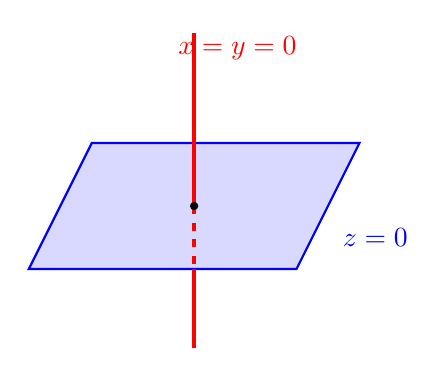
\begin{tikzpicture}[scale=1.0]
  \fill[blue!15] (-2,-0.8)--(1.4,-0.8)--(2.2,0.8)--(-1.2,0.8)--cycle;
  \draw[blue,thick] (-2,-0.8)--(1.4,-0.8)--(2.2,0.8)--(-1.2,0.8)--cycle;
  \draw[very thick,red] (0.1,0)--(0.1,2.2);
  \draw[very thick,red,dashed] (0.1,0)--(0.1,-0.8);
  \draw[very thick,red] (0.1,-0.8)--(0.1,-1.8);
  \node[blue] at (2.4,-0.4) {$z=0$};
  \node[red] at (0.65,2.0) {$x=y=0$};
  \fill (0.1,0) circle (1.5pt);
\end{tikzpicture}
\caption{$\Zero(xz,yz)$：平面と直線の和集合．}
\label{fig:ch03-plane-line}
\end{figure}

\subsection{零点集合の基本性質}

零点集合の基本的な性質をまとめる．$R=k[x_1,\dots,x_n]$ と書く．

\begin{myprop}{零点集合の基本性質}{ch03-zero-props}
$S,T\subset R$，$I,J\subset R$ をイデアルとする．
\begin{enumerate}
  \item（反変性）$S\subset T$ ならば $\Zero(T)\subset\Zero(S)$．
  \item $\Zero(S)=\Zero((S))$．ただし $(S)$ は $S$ で生成されるイデアル．
  \item $\Zero(0)=\A^n$，$\Zero(1)=\emptyset$．
  \item $\Zero(I)\cup\Zero(J)=\Zero(I\cap J)=\Zero(IJ)$．
  \item 任意の族 $\{I_\lambda\}_{\lambda\in\Lambda}$ に対し $\bigcap_\lambda\Zero(I_\lambda)=\Zero\bigl(\sum_\lambda I_\lambda\bigr)$．
\end{enumerate}
\end{myprop}

\begin{proof}
(1) $T$ の全ての元が $P$ で消えれば，$S$ の全ての元も $P$ で消える．

(2) $S\subset(S)$ なので (1) より $\Zero((S))\subset\Zero(S)$．逆に $P\in\Zero(S)$ とする．$(S)$ の元は $g=\sum_i h_if_i$（$h_i\in R$，$f_i\in S$）の形をしており，$g(P)=\sum_i h_i(P)f_i(P)=0$．よって $P\in\Zero((S))$．

(3) 自明．

(4) $IJ\subset I\cap J\subset I$ なので (1) より $\Zero(I)\subset\Zero(I\cap J)\subset\Zero(IJ)$，同様に $\Zero(J)$ についても成り立つから
$\Zero(I)\cup\Zero(J)\subset\Zero(I\cap J)\subset\Zero(IJ)$．
逆に $P\in\Zero(IJ)$ かつ $P\notin\Zero(I)$ とすると，$f(P)\ne0$ となる $f\in I$ がある．任意の $g\in J$ に対し $fg\in IJ$ だから $f(P)g(P)=0$，$k$ は体なので $g(P)=0$．よって $P\in\Zero(J)$．

(5) $P$ が全ての $I_\lambda$ の元で消えることと，それらの有限和 $\sum f_\lambda$ の全てで消えることは同値である．
\end{proof}

(2) により，零点集合を考えるときは多項式の集合 $S$ の代わりにそれが生成するイデアルを考えればよい．
さらに Hilbert の基底定理（第2章）から次が従う．

\begin{myprop}{有限個の方程式で十分}{ch03-finite-gen}
任意の $S\subset k[x_1,\dots,x_n]$ に対し，有限個の $f_1,\dots,f_r\in S$ が存在して $\Zero(S)=\Zero(f_1,\dots,f_r)$ となる．
\end{myprop}

\begin{proof}
$k[x_1,\dots,x_n]$ は Noether 環なので，イデアル $(S)$ は有限生成である．
生成元 $g_1,\dots,g_m$ はそれぞれ $S$ の有限個の元の線形結合で書けるから，それらに現れる $S$ の元を $f_1,\dots,f_r$ とすれば $(S)=(f_1,\dots,f_r)$．
(2) より $\Zero(S)=\Zero((S))=\Zero((f_1,\dots,f_r))=\Zero(f_1,\dots,f_r)$．
\end{proof}

\begin{note}
(4) の等式で $I\cup J$ ではなく $I\cap J$ や $IJ$ が現れることに注意．
「$f=0$ または $g=0$」は「$fg=0$」と同値であるが，これは体（整域）の性質 $ab=0\Rightarrow a=0\text{ または }b=0$ による．
和集合は積に，共通部分は和に対応する：$\Zero(f)\cup\Zero(g)=\Zero(fg)$，$\Zero(f)\cap\Zero(g)=\Zero(f,g)$．
\end{note}

一方，零点集合は多項式の集合を完全には記憶しない．たとえば
\[
  \Zero(x)=\Zero(x^2)=\Zero(x^3)=\cdots=\{0\}\subset\A^1
\]
である．$\Zero$ はイデアルの「冪の違い」を忘れてしまう．この情報の損失を正確に述べたものが第4章の Hilbert の零点定理であり，失われた情報を取り戻す枠組みが第12章のスキーム論である．

\exprob{prob:ch03-3} $\A^2$ において $\Zero(x^2-y,\ x-y)$ と $\Zero(x^2-x,\ xy-y)$ をそれぞれ求めよ．

\exprob{prob:ch03-4} イデアル $I=(x),\ J=(x,y)\subset k[x,y]$ について，$I\cap J$ と $IJ$ を求め，両者が異なるにもかかわらず $\Zero(I\cap J)=\Zero(IJ)$ であることを直接確かめよ．

%======================================================================
\section{代数的集合}
\label{sec:ch03-algset}
%======================================================================

\subsection{代数的集合の定義}

\begin{mydef}{代数的集合}{ch03-algebraic-set}
部分集合 $X\subset\A^n$ が \textbf{(アフィン)代数的集合} (algebraic set) であるとは，
ある多項式の集合 $S\subset k[x_1,\dots,x_n]$ が存在して $X=\Zero(S)$ となることをいう．
命題\ref{prop:ch03-finite-gen}により，このとき $S$ は有限集合に取れる．
\end{mydef}

代数的集合とは「有限個の多項式方程式の共通解として書ける集合」のことである．
文献によってはこれを「アフィン多様体」とよぶこともあるが，本書では既約性などの条件を課したものを第5章で多様体とよぶ．

\begin{myex}{代数的集合の例}{ch03-algset-examples}
\begin{enumerate}
  \item $\A^n=\Zero(0)$，$\emptyset=\Zero(1)$．
  \item 一点 $P=(a_1,\dots,a_n)$：$\{P\}=\Zero(x_1-a_1,\dots,x_n-a_n)$．
  \item 線形部分空間やアフィン部分空間：一次方程式の解集合である．
  \item $\SL_n(k)=\{A\in M_n(k)\mid \det A=1\}\subset\A^{n^2}$ は $\det A-1$ という一つの多項式の零点集合である．
  \item 直交群 $O_n(k)=\{A\mid A^{\mathsf T}A=1\}\subset\A^{n^2}$ は $n(n+1)/2$ 個の二次式の零点集合である．
\end{enumerate}
\end{myex}

一方，代数的集合でない部分集合も多い．

\begin{myex}{代数的集合でない集合}{ch03-not-algset}
\begin{enumerate}
  \item $\Z\subset\A^1_\C$．$\A^1$ の代数的集合は後で見るように有限集合か全体しかない（命題\ref{prop:ch03-A1-closed}）ので，$\Z$ は代数的集合でない．
  \item 正弦曲線 $\Gamma=\{(x,\sin x)\}\subset\A^2_\R$．$\Gamma\subset\Zero(f)$ とする．$-1<c<1$ を満たす任意の $c$ に対し，$\Gamma$ と水平線 $y=c$ の交わりは無限集合なので，一変数多項式 $f(x,c)$ は無限個の根を持ち，恒等的に $0$ である．
        すなわち $f$ は無限本の直線 $y=c$ 上で消える．$f$ を $x$ について整理した各係数（$y$ の多項式）が無限個の根を持つことになるので $f=0$．
        よって $\Gamma$ を含む代数的集合は $\A^2$ 全体のみであり，$\Gamma$ は代数的集合でない．
  \item 上半平面 $\{(x,y)\mid y\ge0\}\subset\A^2_\R$ や単位円板．不等式で定義される集合は（実）代数的集合ではない（半代数的集合とよばれる）．
\end{enumerate}
\end{myex}

\subsection{代数的集合の基本性質}

命題\ref{prop:ch03-zero-props}を代数的集合の言葉で述べ直すと次のようになる．

\begin{mythm}{代数的集合の閉性}{ch03-closed-family}
\begin{enumerate}
  \item $\emptyset$ と $\A^n$ は代数的集合である．
  \item 有限個の代数的集合の和集合は代数的集合である．
  \item 任意個の代数的集合の共通部分は代数的集合である．
\end{enumerate}
\end{mythm}

これは位相空間の閉集合の公理そのものであり，\ref{sec:ch03-zariski}節で Zariski 位相を定義する根拠になる．
無限個の和集合が代数的集合とは限らないことは，$\Z=\bigcup_{m\in\Z}\{m\}\subset\A^1_\C$ の例からわかる．

代数的集合のもう一つの基本性質は \textbf{降鎖条件} である．

\begin{myprop}{代数的集合の降鎖条件}{ch03-dcc}
代数的集合の降鎖 $X_1\supset X_2\supset X_3\supset\cdots$ は必ず有限で止まる．すなわち，ある $N$ があって $X_N=X_{N+1}=\cdots$．
\end{myprop}

\begin{proof}
$X_i$ に対し，$X_i$ 上で消える多項式全体 $\Ideal(X_i)=\{f\mid f|_{X_i}=0\}$ を考えるとこれはイデアルで（第4章で詳しく扱う），
$X_1\supset X_2\supset\cdots$ より $\Ideal(X_1)\subset\Ideal(X_2)\subset\cdots$ はイデアルの昇鎖となる．
$k[x_1,\dots,x_n]$ は Noether 環なので，ある $N$ で $\Ideal(X_N)=\Ideal(X_{N+1})=\cdots$ となる．
一方，代数的集合 $X=\Zero(S)$ について $X=\Zero(\Ideal(X))$ が成り立つ
（$S\subset\Ideal(X)$ より $\Zero(\Ideal(X))\subset\Zero(S)=X$，逆の包含は定義から明らか）．
よって $X_i=\Zero(\Ideal(X_i))$ も $i\ge N$ で一定である．
\end{proof}

\subsection{代数的集合の交}

二つの代数的集合 $X=\Zero(I)$，$Y=\Zero(J)$ の共通部分は
\[
  X\cap Y=\Zero(I+J)=\Zero(I\cup J)
\]
で与えられる．すなわち，方程式を「合併」すればよい．
$I=(f_1,\dots,f_r)$，$J=(g_1,\dots,g_s)$ なら $X\cap Y=\Zero(f_1,\dots,f_r,g_1,\dots,g_s)$ である．

\begin{myex}{放物線と直線の交わり}{ch03-parabola-line}
$\A^2_\C$ において放物線 $X=\Zero(y-x^2)$ と直線 $L_c=\Zero(y-c)$ の交わりは
\[
  X\cap L_c=\Zero(y-x^2,\ y-c)=\Zero(x^2-c,\ y-c)=\{(\pm\sqrt c,\ c)\}
\]
である．$c\ne0$ なら2点，$c=0$ なら1点 $(0,0)$ になる．
$c\to0$ の極限で2点が1点に合流しているので，$c=0$ のときの交点は「重複度2」で数えるのが自然である．
ところが集合としては $\Zero(y-x^2,y)=\Zero(x^2,y)=\Zero(x,y)$ であり，零点集合はこの重複度の情報を失っている．
イデアル $(x^2,y)$ の方は重複度を覚えている（$k[x,y]/(x^2,y)$ が $k$ 上2次元）．これは第9章の交点重複度や第12章のスキームにつながる観点である．
\end{myex}

\begin{figure}[H]
\centering
\begin{tikzpicture}[scale=0.9]
  \draw[->,gray] (-2.2,0)--(2.2,0) node[right]{$x$};
  \draw[->,gray] (0,-0.6)--(0,3.3) node[above]{$y$};
  \draw[very thick,blue,domain=-1.75:1.75,samples=60] plot (\x,{\x*\x});
  \draw[thick,red] (-2.2,1.5)--(2.2,1.5) node[right]{$y=c$};
  \fill[red] ({sqrt(1.5)},1.5) circle (2pt) ({-sqrt(1.5)},1.5) circle (2pt);
  \draw[thick,red,dashed] (-2.2,0.02)--(2.2,0.02);
  \fill[red] (0,0) circle (2pt);
  \node[red,below right] at (0.1,0) {$c=0$：2点が合流};
  \draw[->,red!70] (1.25,1.35)--(0.2,0.2);
\end{tikzpicture}
\caption{放物線と水平線の交わり．$c\to0$ で2つの交点が合流する．}
\label{fig:ch03-parabola-line}
\end{figure}

\subsection{代数的集合の和集合}

和集合については $X\cup Y=\Zero(I\cap J)=\Zero(IJ)$ であった．
生成元で書けば，$I=(f_1,\dots,f_r)$，$J=(g_1,\dots,g_s)$ のとき $IJ=(f_ig_j)_{i,j}$ なので
\[
  X\cup Y=\Zero(f_ig_j\mid 1\le i\le r,\ 1\le j\le s).
\]
「$X$ の方程式が全部成り立つ，または $Y$ の方程式が全部成り立つ」を，積をとることで一つの連立方程式に書き直しているのである．

\begin{myex}{二点の和集合と平面と直線}{ch03-union-examples}
\begin{enumerate}
  \item $\A^1$ の2点 $\{a\}\cup\{b\}=\Zero(x-a)\cup\Zero(x-b)=\Zero((x-a)(x-b))$．
  \item $\A^2$ の2点 $(0,0)$ と $(1,0)$：$\Zero(x,y)\cup\Zero(x-1,y)=\Zero(x(x-1),\ xy,\ y(x-1),\ y^2)$．
        生成元を整理すると $\Zero(x(x-1),\ y)$ に等しい．
  \item 例\ref{ex:ch03-not-ci}の $\Zero(xz,yz)=\Zero(z)\cup\Zero(x,y)$．実際 $(z)\cdot(x,y)=(xz,yz)$ である．
\end{enumerate}
\end{myex}

\subsection{代数的集合の包含関係}

代数的集合の包含関係と多項式の集合の包含関係は \emph{逆向き} に対応する：
方程式を増やせば図形は小さくなる．命題\ref{prop:ch03-zero-props}(1) により $S\subset T\Rightarrow\Zero(T)\subset\Zero(S)$ である．

ただし逆は成り立たない．$\Zero(x^2)\subset\Zero(x)$ であるが $(x)\not\subset(x^2)$．
包含 $\Zero(J)\subset\Zero(I)$ を代数的に判定するには，「$I$ の各元が $\Zero(J)$ 上で消えるか」を調べればよい．
$k$ が代数閉体ならば，これは「$I$ の各元のある冪が $J$ に属するか」，すなわち $I\subset\sqrt{J}$ と同値になる．これが第4章の強零点定理の内容である．

\begin{myex}{包含の判定}{ch03-inclusion}
$X=\Zero(y-x^2)$（放物線），$Y=\Zero(x-1,\ y-1)$（点 $(1,1)$），$Z=\Zero(y^2-x^4)$ とする．
\begin{itemize}
  \item $Y\subset X$：$y-x^2$ に $(1,1)$ を代入すると $0$．
  \item $X\subset Z$：$y^2-x^4=(y-x^2)(y+x^2)\in(y-x^2)$．実際 $Z=X\cup\Zero(y+x^2)$ は二つの放物線の和集合である．
\end{itemize}
したがって $Y\subset X\subset Z$ であり，対応するイデアルは $(y^2-x^4)\subset(y-x^2)\subset(x-1,y-1)$ と逆順に並ぶ．
\end{myex}

\begin{physbox}[真空のモジュライ空間]
超対称ゲージ理論の古典的な真空の集合は，スカラー場 $\phi_i$ の空間の中で F 項条件 $\partial W/\partial\phi_i=0$ と D 項条件で切り出される．
F 項条件は超ポテンシャル $W$ が多項式であれば多項式方程式なので，真空の集合は代数的集合になる．
たとえば $W=\lambda\,\phi\,(\chi^2-v^2)$ なら F 項条件は $\chi^2-v^2=0$，$2\phi\chi=0$ であり，真空は $\Zero(\chi^2-v^2,\ \phi\chi)=\{(\phi,\chi)=(0,\pm v)\}$ の2点である．
$v\to0$ とすると F 項条件は $\chi^2=0,\ \phi\chi=0$ となり，真空の集合は直線 $\{\chi=0\}$（平坦方向）へと大きく変化する．
「方程式の係数を動かすと解集合の形が飛ぶ」という現象は，代数的集合の族として理解される．
\end{physbox}

\exprob{prob:ch03-5} $\A^2$ の3点 $(0,0),(1,0),(0,1)$ からなる集合を，二次式のみを用いた連立方程式の零点集合として表せ．

\exprob{prob:ch03-6} 集合 $\{(x,y)\in\A^2_\C\mid y=e^x\}$ が代数的集合でないことを示せ．（ヒント：直線 $y=1$ との交わりを考えよ．）

%======================================================================
\section{Zariski位相}
\label{sec:ch03-zariski}
%======================================================================

\subsection{位相空間の復習}

集合 $X$ の部分集合の族 $\mathcal{O}$ が次を満たすとき，$\mathcal O$ を $X$ の \textbf{位相} といい，$\mathcal O$ の元を \textbf{開集合} という：
\begin{enumerate}
  \item $\emptyset,\ X\in\mathcal O$，
  \item 任意個の開集合の和集合は開集合，
  \item 有限個の開集合の共通部分は開集合．
\end{enumerate}
開集合の補集合を \textbf{閉集合} という．De Morgan の法則により，閉集合の族 $\mathcal F$ は
(i) $\emptyset,X\in\mathcal F$，(ii) 有限個の和集合で閉じる，(iii) 任意個の共通部分で閉じる，を満たし，
逆にこれらを満たす族 $\mathcal F$ を閉集合系として位相が一意に定まる．

部分集合 $A\subset X$ の \textbf{閉包} $\overline{A}$ は $A$ を含む最小の閉集合（$A$ を含む閉集合全ての共通部分）である．
$\overline A=X$ のとき $A$ は \textbf{稠密} であるという．
$X$ が \textbf{Hausdorff} であるとは，任意の異なる2点 $P\ne Q$ に対し，互いに交わらない開集合 $U\ni P$，$V\ni Q$ が存在することをいう．
$X$ が \textbf{準コンパクト} であるとは，任意の開被覆が有限部分被覆を持つことをいう（Hausdorff を仮定しないコンパクト性）．
部分集合 $Y\subset X$ には $\{U\cap Y\mid U\in\mathcal O\}$ を開集合系とする \textbf{相対位相} が入る．

物理学で普段使う $\R^n$ や $\C^n$ の位相（Euclid 位相）は距離から定まる位相であり，Hausdorff である．
以下ではこれを \textbf{通常の位相}（あるいは古典位相，複素位相）とよび，Zariski 位相と区別する．

\subsection{Zariski閉集合}

\begin{mydef}{Zariski閉集合}{ch03-zariski-closed}
$\A^n$ の代数的集合，すなわち $\Zero(S)$ の形の部分集合を \textbf{Zariski閉集合} という．
\end{mydef}

定理\ref{thm:ch03-closed-family}により，Zariski閉集合の全体は閉集合系の公理 (i)--(iii) を満たす．
より一般に，代数的集合 $X\subset\A^n$ に対し，$X$ に含まれる代数的集合を $X$ の Zariski 閉集合という．

\subsection{Zariski位相の定義}

\begin{mydef}{Zariski位相}{ch03-zariski}
Zariski閉集合全体を閉集合系とする $\A^n$ の位相を \textbf{Zariski位相} (Zariski topology) という．
代数的集合 $X\subset\A^n$ には，その相対位相を入れ，これを $X$ の Zariski 位相とよぶ．
$X$ の閉集合はちょうど $X$ に含まれる代数的集合であり，$X\cap\Zero(S)=\Zero(\Ideal(X)\cup S)$ の形をしている．
\end{mydef}

Zariski位相は「多項式関数が連続になる最も粗い位相」（ただし $k$ に有限集合と全体のみを閉集合とする位相を入れる）と言い換えることもできる．
実際，多項式 $f$ に対し $f^{-1}(c)=\Zero(f-c)$ は閉集合だからである．

\begin{myprop}{$\A^1$ のZariski位相}{ch03-A1-closed}
$k$ を無限体とする．$\A^1$ の Zariski 閉集合は，$\A^1$ 自身と有限部分集合（空集合を含む）に限る．
したがって $\A^1$ の空でない開集合は有限個の点を除いた集合（補有限集合）である．
\end{myprop}

\begin{proof}
$X=\Zero(S)$，$S\subset k[x]$ とする．$S\subset\{0\}$ ならば $X=\A^1$．
$S$ が零でない $f$ を含めば $X\subset\Zero(f)$ であり，$\Zero(f)$ は $f$ の根の集合で高々 $\deg f$ 個の元からなる．よって $X$ は有限集合．
逆に有限集合 $\{a_1,\dots,a_m\}=\Zero\bigl(\prod_i(x-a_i)\bigr)$ は閉集合である．
\end{proof}

つまり $\A^1$ の Zariski 位相は \textbf{補有限位相} (cofinite topology) にほかならない．
$\A^1_\C=\C$ で言えば，通常の位相で閉である円周 $|z|=1$ や実軸 $\R\subset\C$ も，Zariski 位相では閉集合ではない．
実軸を含む最小の Zariski 閉集合は $\C$ 全体，すなわち $\R$ は $\A^1_\C$ で \emph{Zariski 稠密} である．

\subsection{Zariski開集合}

Zariski 閉集合の補集合を \textbf{Zariski開集合} という．特に重要なのは一つの多項式で定まる開集合である．

\begin{mydef}{基本開集合}{ch03-basic-open}
$f\in k[x_1,\dots,x_n]$ に対し
\[
  D(f):=\A^n\setminus\Zero(f)=\{P\in\A^n\mid f(P)\ne0\}
\]
を \textbf{基本開集合} (basic open set, principal open set) という．
\end{mydef}

\begin{myprop}{基本開集合は開基をなす}{ch03-basis}
\begin{enumerate}
  \item $D(f)\cap D(g)=D(fg)$．
  \item $\A^n$ の任意の Zariski 開集合は有限個の基本開集合の和集合である．
\end{enumerate}
特に基本開集合全体は Zariski 位相の開基をなす．
\end{myprop}

\begin{proof}
(1) $f(P)g(P)\ne0\iff f(P)\ne0$ かつ $g(P)\ne0$．
(2) 開集合 $U$ に対し $\A^n\setminus U=\Zero(f_1,\dots,f_r)$（命題\ref{prop:ch03-finite-gen}）と書けるので，
$U=\A^n\setminus\bigcap_i\Zero(f_i)=\bigcup_i D(f_i)$．
\end{proof}

\begin{myex}{開集合の例}{ch03-open-examples}
\begin{enumerate}
  \item $D(x)=\A^1\setminus\{0\}$．これは $k^\times$ であり，物理では「$\C^\times$ 上の理論」として頻出する．
  \item $\GL_n(k)=D(\det)\subset\A^{n^2}$．可逆行列全体は Zariski 開集合である．
  \item $\A^2$ から原点を除いた $U=\A^2\setminus\{(0,0)\}=D(x)\cup D(y)$．$U$ は基本開集合ではない（$\{(0,0)\}=\Zero(f)$ となる多項式 $f$ は存在しない．$k$ が代数閉なら $\Zero(f)$ は空か1次元だからである）．
\end{enumerate}
\end{myex}

\begin{physbox}[一般の点と特別な点]
物理でパラメータ空間を考えるとき，「一般的な (generic) パラメータでは対称性が破れていて，特別な値でのみ対称性が回復する」という状況がよく現れる．
たとえば行列 $M$ の固有値が縮退する条件は判別式 $\Delta(M)=0$ という多項式方程式で書ける．
このとき縮退が起こる点の集合 $\Zero(\Delta)$ は Zariski 閉集合であり，縮退しない点の集合 $D(\Delta)$ は Zariski 開かつ稠密である．
物理学者の言う「generic」とは，多くの場合「空でない Zariski 開集合に属する」ことを意味すると考えてよい．
\end{physbox}

\subsection{Zariski位相と通常の位相の比較}

$k=\C$ とする．多項式は連続関数なので，$\Zero(f)=f^{-1}(0)$ は通常の位相で閉集合であり，その任意個の共通部分も閉である．したがって

\begin{myprop}{Zariski位相は通常の位相より粗い}{ch03-coarser}
$\A^n_\C$ の Zariski 閉（開）集合は通常の位相でも閉（開）である．逆は成り立たない．
\end{myprop}

逆が成り立たない例は，閉円板 $\{|z|\le1\}\subset\C$ や実軸 $\R\subset\C$ である．
Zariski 開集合は「非常に大きい」：空でない Zariski 開集合は通常の位相で稠密である（例えば $D(f)$ は超曲面 $\Zero(f)$ を除いた集合であり，$\Zero(f)$ は内点を持たない）．

最も顕著な違いは次の性質である．

\begin{myprop}{非Hausdorff性}{ch03-non-hausdorff}
$k$ を無限体，$n\ge1$ とする．$\A^n$ の任意の二つの空でない Zariski 開集合は交わる．
特に $\A^n$ は Hausdorff でない．
\end{myprop}

\begin{proof}
空でない開集合 $U,V$ は基本開集合 $D(f)\subset U$，$D(g)\subset V$（$f,g\ne0$）を含む．
$D(f)\cap D(g)=D(fg)$ であり，$fg\ne0$ なので命題\ref{prop:ch03-poly-function}により $fg(P)\ne0$ となる点 $P$ が存在する．よって $U\cap V\ne\emptyset$．
\end{proof}

図\ref{fig:ch03-nonhausdorff}は $\A^1$ における状況を示している．
二点 $P,Q$ を分離しようとして $P$ の開近傍 $U$ を取っても，$U$ は有限個の点を除いた全体なので，$Q$ のどんな開近傍とも（実際無限個の点で）交わってしまう．

\begin{figure}[H]
\centering
\begin{tikzpicture}[scale=1.0]
  \begin{scope}
    \node at (2.5,1.2) {通常の位相（Hausdorff）};
    \draw[thick] (0,0)--(5,0);
    \fill (1.5,0) circle (2pt) node[below]{$P$};
    \fill (3.5,0) circle (2pt) node[below]{$Q$};
    \draw[blue,thick] (1.5,0) ellipse (0.6 and 0.3);
    \draw[red,thick] (3.5,0) ellipse (0.6 and 0.3);
    \node[blue] at (1.5,0.55) {$U$}; \node[red] at (3.5,0.55) {$V$};
  \end{scope}
  \begin{scope}[xshift=7cm]
    \node at (2.5,1.2) {Zariski位相};
    \draw[blue,line width=3pt,opacity=0.35] (0,0.08)--(5,0.08);
    \draw[red,line width=3pt,opacity=0.35] (0,-0.08)--(5,-0.08);
    \foreach \t in {0.6,2.6,4.3} {\fill[white] (\t,0.08) circle (2.5pt); \draw[blue] (\t,0.08) circle (2.5pt);}
    \foreach \t in {1.1,3.1,4.0} {\fill[white] (\t,-0.08) circle (2.5pt); \draw[red] (\t,-0.08) circle (2.5pt);}
    \fill (1.5,0) circle (2pt) node[below=3pt]{$P$};
    \fill (3.5,0) circle (2pt) node[below=3pt]{$Q$};
    \node[blue] at (0.3,0.45) {$U$}; \node[red] at (0.3,-0.45) {$V$};
  \end{scope}
\end{tikzpicture}
\caption{$\A^1$ における点の分離．Zariski 開集合は有限個の点（白丸）を除いた全体なので，$P$ と $Q$ の近傍は必ず交わる．}
\label{fig:ch03-nonhausdorff}
\end{figure}

\paragraph{$\A^2$ の位相は $\A^1\times\A^1$ の積位相ではない．}
集合としては $\A^2=\A^1\times\A^1$ であるが，Zariski 位相は積位相より真に細かい．
積位相における閉集合は，$\A^1$ の閉集合（有限集合または全体）の積 $F_1\times F_2$ の有限和とその任意の共通部分である．
具体的には，積位相の閉集合は「有限個の点，有限個の水平線 $\{y=b\}$，有限個の垂直線 $\{x=a\}$」の和集合（および全体）に限られる．
ところが対角線 $\Delta=\Zero(x-y)$ や放物線 $\Zero(y-x^2)$ は Zariski 閉集合であるが，積位相では閉でない（図\ref{fig:ch03-product}）．
これは，代数幾何学では「直積」を位相の直積として定義してはならないことを示している．
正しい直積は座標環のテンソル積 $k[x]\otimes_k k[y]=k[x,y]$ に基づいて定義される（第5章，第12章）．

\begin{figure}[H]
\centering
\begin{tikzpicture}[scale=0.9]
  \begin{scope}
    \draw[->,gray] (-0.2,0)--(3.4,0); \draw[->,gray] (0,-0.2)--(0,3.4);
    \draw[thick,blue] (0.8,-0.2)--(0.8,3.3);
    \draw[thick,blue] (2.3,-0.2)--(2.3,3.3);
    \draw[thick,blue] (-0.2,1.9)--(3.3,1.9);
    \fill[blue] (1.6,0.7) circle (2pt);
    \node at (1.6,-0.8) {積位相の閉集合};
  \end{scope}
  \begin{scope}[xshift=5.5cm]
    \draw[->,gray] (-0.2,0)--(3.4,0); \draw[->,gray] (0,-0.2)--(0,3.4);
    \draw[thick,red] (-0.2,-0.2)--(3.3,3.3) node[right]{$x=y$};
    \draw[thick,red,domain=0:1.8,samples=40] plot (\x,{\x*\x});
    \node[red] at (2.4,3.2) {$y=x^2$};
    \node at (1.6,-0.8) {Zariski 閉だが積位相で閉でない};
  \end{scope}
\end{tikzpicture}
\caption{$\A^1\times\A^1$ の積位相と $\A^2$ の Zariski 位相．}
\label{fig:ch03-product}
\end{figure}

\subsection{Zariski位相の特徴}

Zariski 位相の主な特徴をまとめておく．

\begin{myprop}{Zariski位相の性質}{ch03-zariski-props}
$X\subset\A^n$ を代数的集合とし，Zariski 位相を入れる．
\begin{enumerate}
  \item（$T_1$ 性）一点集合は閉集合である．
  \item（Noether性）$X$ の閉集合の降鎖は有限で止まる．同値なことに開集合の昇鎖は有限で止まる．
  \item（準コンパクト性）$X$ の任意の部分集合は準コンパクトである．
  \item 多項式写像 $\varphi\colon\A^n\to\A^m$，$P\mapsto(\varphi_1(P),\dots,\varphi_m(P))$ は Zariski 位相について連続である．
\end{enumerate}
\end{myprop}

\begin{proof}
(1) 例\ref{ex:ch03-algset-examples}(2)．(2) 命題\ref{prop:ch03-dcc}．

(3) $Y\subset X$ と $Y$ の開被覆 $\{U_\lambda\}$ を取る．有限個の $U_\lambda$ の和集合全体の族を考えると，(2) より（開集合の昇鎖条件から）この族には包含に関する極大元 $U=U_{\lambda_1}\cup\cdots\cup U_{\lambda_r}$ が存在する（極大元がなければ真の昇鎖が無限に作れる）．
もし $U\ne Y$ なら $U\cup U_\mu\supsetneq U$ となる $U_\mu$ があり極大性に反する．よって $U=Y$．

(4) 閉集合 $\Zero(g_1,\dots,g_s)\subset\A^m$ の逆像は $\Zero(g_1\circ\varphi,\dots,g_s\circ\varphi)$ であり，$g_j\circ\varphi$ は多項式なので閉集合である．
\end{proof}

(3) の準コンパクト性は，$\C^n$ が通常の位相ではコンパクトでないことと対照的である．Zariski 位相では「開集合が大きすぎる」ためにこのような現象が起こる．

\begin{note}
Zariski 位相は粗すぎるため，通常の位相で使える議論（たとえば陰関数定理や，点の小さな近傍での議論）はそのままでは使えない．
その代わりに代数幾何学では，局所環（第6章）や接空間（第7章）といった代数的な道具で「局所的」な性質を捉える．
一方，「空でない開集合は稠密」という性質は，「ある一点で成り立つ開条件は一般の点で成り立つ」という強力な原理を与える．
\end{note}

\exprob{prob:ch03-7} $\A^1$ の部分集合 $A$ の Zariski 閉包を求めよ：(a) $A=\{1,2,3\}$，(b) $A=\Z$（$k=\C$），(c) $A=\{z\in\C\mid|z|=1\}$．

\exprob{prob:ch03-8} $\A^2_\C$ において，集合 $\{(t,t^2)\mid t\in\R\}$ の Zariski 閉包を求めよ．

%======================================================================
\section{既約性}
\label{sec:ch03-irred}
%======================================================================

\subsection{既約な位相空間}

$\Zero(xy)$ は二本の直線の和集合であり，「二つの部分に分かれている」．
一方，通常の位相では $\Zero(xy)$ は連結である．
連結性とは別の意味での「分かれ方」を捉えるのが既約性である．

\begin{mydef}{既約な位相空間}{ch03-irreducible-space}
位相空間 $X$ が \textbf{既約} (irreducible) であるとは，$X\ne\emptyset$ であり，
$X=X_1\cup X_2$（$X_1,X_2$ は閉集合）と書けるならば $X=X_1$ または $X=X_2$ となることをいう．
既約でない空でない空間を \textbf{可約} (reducible) という．
部分集合 $Y\subset X$ が既約であるとは，相対位相で既約であることをいう．
\end{mydef}

\begin{mylem}{既約性の言い換え}{ch03-irred-equiv}
空でない位相空間 $X$ について次は同値である．
\begin{enumerate}
  \item $X$ は既約．
  \item 任意の二つの空でない開集合 $U,V\subset X$ は交わる．
  \item 任意の空でない開集合は $X$ で稠密である．
\end{enumerate}
\end{mylem}

\begin{proof}
(1)$\Rightarrow$(2)：$U\cap V=\emptyset$ ならば $X=(X\setminus U)\cup(X\setminus V)$ で，既約性から $X\setminus U=X$ または $X\setminus V=X$，すなわち $U$ か $V$ が空．
(2)$\Rightarrow$(3)：$U$ が稠密でなければ $V=X\setminus\overline U$ は空でない開集合で $U\cap V=\emptyset$．
(3)$\Rightarrow$(1)：$X=X_1\cup X_2$（閉）で $X_1\ne X$ とすると，$U=X\setminus X_1$ は空でない開集合で $U\subset X_2$．$U$ は稠密なので $X=\overline U\subset X_2$．
\end{proof}

Hausdorff 空間で既約なのは一点だけである（二点あれば分離する開集合が取れるから）．したがって既約性は Zariski 位相のような非 Hausdorff な位相に特有の概念である．
命題\ref{prop:ch03-non-hausdorff}は，まさに「$\A^n$ は既約である」と言っている．

\begin{mylem}{既約性の基本性質}{ch03-irred-basic}
$X$ を位相空間とする．
\begin{enumerate}
  \item $Y\subset X$ が既約ならば，その閉包 $\overline Y$ も既約．
  \item 既約空間の空でない開集合は既約かつ稠密．
  \item $X$ が既約で $f\colon X\to Z$ が連続ならば，$f(X)$ は既約．
\end{enumerate}
\end{mylem}

\begin{proof}
(1) $\overline Y=F_1\cup F_2$（閉）なら $Y=(Y\cap F_1)\cup(Y\cap F_2)$ で，$Y$ の既約性から例えば $Y\subset F_1$．$F_1$ は閉なので $\overline Y\subset F_1$．
(2) 補題\ref{lem:ch03-irred-equiv}(2) を開集合 $U$ に適用すればよい（$U$ の開集合は $X$ の開集合でもある）．
(3) $f(X)=F_1\cup F_2$（$f(X)$ の閉集合）なら $X=f^{-1}(F_1)\cup f^{-1}(F_2)$ で，例えば $X=f^{-1}(F_1)$，よって $f(X)=F_1$．
\end{proof}

\subsection{既約代数的集合}

代数的集合 $X\subset\A^n$ が既約であるとは，Zariski 位相について既約であること，すなわち
\[
  X=X_1\cup X_2\ (X_i\text{ は代数的集合})\ \Longrightarrow\ X=X_1\ \text{または}\ X=X_2
\]
が成り立つことである．直感的には「これ以上真に小さい代数的集合の和に分けられない図形」である．

\begin{myex}{既約・可約の例}{ch03-irred-ex}
\begin{enumerate}
  \item 一点は既約．$\A^n$ は既約（命題\ref{prop:ch03-non-hausdorff}と補題\ref{lem:ch03-irred-equiv}）．
  \item $\Zero(xy)=\Zero(x)\cup\Zero(y)$ は可約．
  \item 有限集合は点が2個以上あれば可約．
  \item 放物線 $C=\Zero(y-x^2)$ は既約．実際，$\varphi\colon\A^1\to\A^2$，$t\mapsto(t,t^2)$ は多項式写像で連続（命題\ref{prop:ch03-zariski-props}(4)），像は $C$．$\A^1$ が既約なので補題\ref{lem:ch03-irred-basic}(3) から $C$ も既約．
\end{enumerate}
\end{myex}

例 (4) の議論は一般化できる：\textbf{多項式でパラメータ付けされる集合は既約である}．
ねじれ3次曲線 $t\mapsto(t,t^2,t^3)$ や尖点曲線 $t\mapsto(t^2,t^3)$ の像も既約である．
（像が閉集合であることは別途確認が要るが，これらの例では像はちょうど $\Zero(y-x^2,z-x^3)$，$\Zero(y^2-x^3)$ に一致する．）

\subsection{既約成分}

\begin{mydef}{既約成分}{ch03-irred-component}
位相空間 $X$ の既約部分集合のうち，包含関係について極大なものを $X$ の \textbf{既約成分} (irreducible component) という．
\end{mydef}

補題\ref{lem:ch03-irred-basic}(1) より，既約成分は必ず閉集合である（$\overline Y$ も既約で $Y\subset\overline Y$ なので極大性より $Y=\overline Y$）．
また，任意の既約部分集合はある既約成分に含まれる（Zorn の補題による；既約集合の鎖の和は既約である）．

\begin{myex}{既約成分の例}{ch03-component-ex}
\begin{enumerate}
  \item $\Zero(xy)\subset\A^2$ の既約成分は二直線 $\Zero(x)$ と $\Zero(y)$．
  \item $\Zero(xz,yz)\subset\A^3$ の既約成分は平面 $\Zero(z)$ と直線 $\Zero(x,y)$（例\ref{ex:ch03-not-ci}）．次元の異なる成分が共存しうる．
  \item 有限集合の既約成分は各点．
\end{enumerate}
\end{myex}

既約成分どうしは交わってよい（例 (1) の原点）．この点が連結成分との大きな違いである．
連結成分は互いに交わらないが，既約成分は「部品どうしが接着されている」状況を表現できる．

\subsection{既約分解}

\begin{mydef}{Noether位相空間}{ch03-noetherian-space}
位相空間 $X$ の閉集合の任意の降鎖 $Z_1\supset Z_2\supset\cdots$ が有限で止まるとき，$X$ を \textbf{Noether位相空間} という．
\end{mydef}

命題\ref{prop:ch03-zariski-props}(2) により，代数的集合は Zariski 位相で Noether 位相空間である．
Noether 性は次の \textbf{Noether 帰納法} を可能にする：
\begin{quote}
$X$ の閉集合の空でない族 $\Sigma$ は包含関係について極小元を持つ．
\end{quote}
（極小元がなければ $Z_1\supsetneq Z_2\supsetneq\cdots$ と無限降鎖が作れてしまう．）

\begin{mythm}{既約分解の存在と一意性}{ch03-irred-decomp}
$X$ を空でない Noether 位相空間とする．このとき $X$ は有限個の既約閉集合の和
\[
  X=X_1\cup X_2\cup\cdots\cup X_r,\qquad X_i\not\subset X_j\ (i\ne j)
\]
として表され，このような表示（\textbf{無駄のない既約分解}）は順序を除いて一意である．
さらに $X_1,\dots,X_r$ はちょうど $X$ の既約成分の全体である．
特に，任意の代数的集合は有限個の既約代数的集合の無駄のない和として一意的に表される．
\end{mythm}

\begin{proof}
\textbf{存在．}有限個の既約閉集合の和として書けない空でない閉集合 $Z\subset X$ の族を $\Sigma$ とし，$\Sigma\ne\emptyset$ と仮定する．
Noether 性から $\Sigma$ は極小元 $Z$ を持つ．$Z$ は既約ではない（既約ならそれ自身が1個の和）から，$Z=Z'\cup Z''$（$Z',Z''\subsetneq Z$ は閉）と書ける．
$Z',Z''$ は空でない（空なら他方が $Z$ に等しい）．極小性から $Z',Z''\notin\Sigma$ なので，それぞれ有限個の既約閉集合の和であり，したがって $Z$ もそうである．矛盾．
よって $X$ は $X=X_1\cup\cdots\cup X_r$（$X_i$ 既約閉）と書ける．$X_i\subset X_j$（$i\ne j$）となるものがあれば $X_i$ を取り除けばよいので，無駄のない表示が得られる．

\textbf{一意性．}$X=X_1\cup\cdots\cup X_r=Y_1\cup\cdots\cup Y_s$ を二つの無駄のない既約分解とする．
$X_1=\bigcup_j(X_1\cap Y_j)$ であり，$X_1\cap Y_j$ は $X_1$ の閉集合なので，$X_1$ の既約性から $X_1\subset Y_j$ となる $j$ がある（有限和への帰納的適用）．
同様に $Y_j\subset X_i$ となる $i$ があり，$X_1\subset Y_j\subset X_i$．無駄のなさから $i=1$，よって $X_1=Y_j$．
これを全ての $X_i$ に行えば $\{X_i\}\subset\{Y_j\}$，対称性から逆も成り立つ．

\textbf{既約成分との一致．}$Y\subset X$ が既約ならば，上と同じ議論で $Y\subset X_i$ となる $i$ がある．
したがって極大な既約部分集合は $X_i$ のいずれかに一致する．逆に各 $X_i$ が極大であることは，$X_i\subset Y$（$Y$ 既約）なら $Y\subset X_j$ となる $j$ があり $X_i\subset X_j$，よって $i=j$ かつ $Y=X_i$ となることからわかる．
\end{proof}

\begin{figure}[H]
\centering
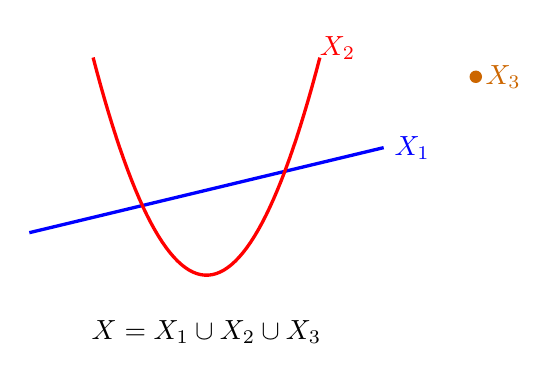
\begin{tikzpicture}[scale=0.9]
  \draw[very thick,blue] (-2.5,-0.6) -- (2.5,0.6) node[right]{$X_1$};
  \draw[very thick,red,domain=-1.6:1.6,samples=60] plot (\x,{1.2*\x*\x-1.2}) ;
  \node[red] at (1.85,2.0) {$X_2$};
  \fill[orange!80!black] (3.8,1.6) circle (2.5pt) node[right]{$X_3$};
  \node at (0,-2.0) {$X=X_1\cup X_2\cup X_3$};
\end{tikzpicture}
\caption{既約分解の模式図．直線 $X_1$，曲線 $X_2$，孤立点 $X_3$．既約成分は交わってもよく，次元が異なってもよい．}
\label{fig:ch03-decomp}
\end{figure}

図\ref{fig:ch03-decomp}のような集合は例えば
$X=\Zero(y)\cup\Zero(y-x^2+1)\cup\{(3,1)\}$ として実現される．

\subsection{既約性と整域}

既約性を多項式の言葉で特徴づけよう．代数的集合 $X\subset\A^n$ に対し
\[
  \Ideal(X):=\{f\in k[x_1,\dots,x_n]\mid \text{全ての } P\in X \text{ で } f(P)=0\}
\]
を $X$ の \textbf{消滅イデアル} とよぶ．
$\Ideal(X)$ がイデアルであることは容易に確かめられる．消滅イデアルの詳しい性質は第4章で扱う．
ここで必要なのは次の二つだけである（命題\ref{prop:ch03-dcc}の証明で示した）：
\[
  X\subset Y\Rightarrow \Ideal(Y)\subset\Ideal(X),\qquad X=\Zero(\Ideal(X))\quad(X\text{ は代数的集合}).
\]
後者から，代数的集合については $X\subsetneq Y\Rightarrow\Ideal(Y)\subsetneq\Ideal(X)$ が従う．

\begin{mythm}{既約性と素イデアル}{ch03-irred-prime}
代数的集合 $X\subset\A^n$ について，次は同値である．
\begin{enumerate}
  \item $X$ は既約である．
  \item $\Ideal(X)$ は素イデアルである．
  \item 剰余環 $k[X]:=k[x_1,\dots,x_n]/\Ideal(X)$ は整域である．
\end{enumerate}
\end{mythm}

\begin{proof}
(2)$\Leftrightarrow$(3) は素イデアルの定義と剰余環の性質（第2章）から直ちに従う．

(1)$\Rightarrow$(2)：$X\ne\emptyset$ なので $1\notin\Ideal(X)$．$fg\in\Ideal(X)$ とすると
$X\subset\Zero(fg)=\Zero(f)\cup\Zero(g)$ なので
\[
  X=(X\cap\Zero(f))\cup(X\cap\Zero(g))
\]
は閉集合二つの和．既約性から，例えば $X=X\cap\Zero(f)$，すなわち $f$ は $X$ 上で消え $f\in\Ideal(X)$．

(2)$\Rightarrow$(1)：$\Ideal(X)$ は真のイデアルなので $X\ne\emptyset$（$\Ideal(\emptyset)=k[x_1,\dots,x_n]$）．
$X=X_1\cup X_2$（$X_i$ は代数的集合）で $X_1\ne X$，$X_2\ne X$ と仮定する．
上の注意から $\Ideal(X)\subsetneq\Ideal(X_i)$ なので，$f_i\in\Ideal(X_i)\setminus\Ideal(X)$ が取れる．
すると $f_1f_2$ は $X_1$ 上でも $X_2$ 上でも消えるので $f_1f_2\in\Ideal(X)$．しかし $f_1,f_2\notin\Ideal(X)$ であり，$\Ideal(X)$ が素であることに反する．
\end{proof}

剰余環 $k[X]$ は $X$ の \textbf{座標環} とよばれ，$X$ 上の多項式関数の環とみなせる（第4章で導入し，第5章で詳しく扱う）．
定理\ref{thm:ch03-irred-prime}は
\begin{center}
「図形が二つに分かれる」$\iff$「零でない二つの関数の積が零になる」
\end{center}
という直感的な対応を述べている．実際 $X=\Zero(xy)$ 上では関数 $x$ と $y$ はどちらも恒等的に $0$ ではないが，積 $xy$ は $X$ 上で恒等的に $0$ である：$x$ は直線 $\Zero(y)$ 上でのみ非零，$y$ は直線 $\Zero(x)$ 上でのみ非零で，台が別々の成分に分かれている．

\begin{physbox}[Higgs branch と Coulomb branch]
超対称ゲージ理論の真空のモジュライ空間は，しばしば複数の既約成分からなる．
典型例は，ゲージ不変量で書いたときに $\Zero(xy)\subset\A^2$ のような形になる場合である：
一方の成分（$y=0$，$x$ が自由）ではベクトル多重項のスカラー $x$ が値を持ち，ゲージ群は可換な部分群（Cartan部分群）までしか破れない（Coulomb branch に相当）．
もう一方の成分（$x=0$）ではハイパー多重項のスカラーが値を持ちゲージ群が Higgs 機構で破れる（Higgs branch に相当）．
二つの既約成分は原点で交わり，そこでは余分な粒子が質量ゼロになる．
既約分解は，「物理的に異なる相（branch）が何個あり，どこで接続しているか」を数学的に記述する言語である．
\end{physbox}

\exprob{prob:ch03-9} $X=\Zero(x^2-yz,\ xz-x)\subset\A^3$ の既約分解を求めよ．

\exprob{prob:ch03-10} 既約な位相空間は連結であることを示せ．また，連結だが既約でない代数的集合の例を挙げよ．

%======================================================================
\section{代数的集合の具体例}
%======================================================================

本節では，これまでの概念を具体例で確認する．以下 $k$ は代数閉体で，$\mathrm{char}\,k\ne2$ とする（二次形式の標準形を使うため）．

\subsection{直線と平面}

$\A^n$ の \textbf{アフィン部分空間}（直線・平面・超平面など）は一次方程式系
\[
  \sum_{j=1}^n a_{ij}x_j=b_i\qquad(i=1,\dots,r)
\]
の解集合である．解が存在すれば，それは $d=n-\rank(a_{ij})$ 次元のパラメータ表示
\[
  \bm x=\bm p+t_1\bm v_1+\cdots+t_d\bm v_d
\]
を持つ．これは多項式（一次式）写像 $\A^d\to\A^n$ の像であり，$\A^d$ が既約なので，\textbf{アフィン部分空間は既約} である．
また消滅イデアルは一次式で生成される素イデアルであり，座標を取り替えれば $(x_{d+1},\dots,x_n)$ の形になる．
このとき座標環は $k[x_1,\dots,x_n]/(x_{d+1},\dots,x_n)\cong k[x_1,\dots,x_d]$，すなわち $d$ 次元アフィン空間の座標環である．

\begin{myex}{二平面の交わり}{ch03-two-planes}
$\A^3$ の二平面 $H_1=\Zero(x+y+z-1)$，$H_2=\Zero(x-y)$ の交わりは
\[
  H_1\cap H_2=\Zero(x+y+z-1,\ x-y)=\{(t,\ t,\ 1-2t)\mid t\in k\}
\]
という直線である．平行な二平面 $\Zero(z)$ と $\Zero(z-1)$ の交わりは $\Zero(z,z-1)=\Zero(1)=\emptyset$ である．
このように，アフィン空間では「平行なものは交わらない」という例外が生じる．射影空間（第8章）に移るとこの例外が消える．
\end{myex}

\subsection{二次曲線}

$\A^2$ の二次曲線は $f(x,y)=ax^2+bxy+cy^2+dx+ey+g=0$（$(a,b,c)\ne0$）で定義される．
$k$ が代数閉体ならば，アフィン変換により $f$ は次のいずれかの標準形に変換できる：
\begin{center}
\begin{tabular}{lll}
標準形 & 名前 & 既約性 \\ \hline
$xy-1$ （または $x^2+y^2-1$） & 非退化中心二次曲線 & 既約 \\
$y-x^2$ & 放物線 & 既約 \\
$xy$ & 交わる二直線 & 可約 \\
$x^2-1$ & 平行な二直線 & 可約 \\
$x^2$ & 二重直線 & 既約（集合として直線）
\end{tabular}
\end{center}
代数閉体上では楕円と双曲線の区別は消える：$k=\C$ で $u=x+iy$，$v=x-iy$ と置けば $x^2+y^2-1=uv-1$ である．
実際，実の円 $x^2+y^2=1$ の複素化は，$\C^2$ の中では双曲線 $uv=1$ と同型な曲線で，これは $\C^\times$ と同型である（$u\in\C^\times$ を与えれば $v=1/u$）．

\begin{myex}{双曲線の既約性}{ch03-hyperbola}
$X=\Zero(xy-1)$ は既約である．実際，$\varphi\colon D(t)=\A^1\setminus\{0\}\to\A^2$，$t\mapsto(t,1/t)$ の像は $X$ であり，
$D(t)$ は既約空間 $\A^1$ の空でない開集合なので既約（補題\ref{lem:ch03-irred-basic}(2)），$\varphi$ は連続（$\Zero(g(x,y))$ の逆像は $t^Ng(t,1/t)=0$ の解集合で閉）．
よって補題\ref{lem:ch03-irred-basic}(3) から $X$ は既約．代数的には $xy-1$ が既約多項式であること（次の\ref{subsec:ch03-irred-test}小節）からも従う．
\end{myex}

二重直線 $\Zero(x^2)$ は集合としては直線 $\Zero(x)$ と同じであるが，方程式 $x^2$ は「直線を二重に数える」情報を持っている．
退化した二次曲線の族 $x^2-\epsilon^2=0$（平行二直線 $x=\pm\epsilon$）の $\epsilon\to0$ の極限が二重直線である．
この「重複度」は零点集合だけでは見えない情報であり，第12章でスキームとして扱われる．

\subsection{二次曲面}

$\A^3$ の二次曲面 $\Zero(q)$，$q$ は二次多項式，を考える．
斉次二次形式 $q(x,y,z)$ はランクによって分類され，代数閉体上では標準形
\[
  \text{rank }3:\ x^2+y^2+z^2,\qquad \text{rank }2:\ x^2+y^2,\qquad \text{rank }1:\ x^2
\]
を持つ．
\begin{itemize}
  \item \textbf{rank 3：二次錐面} $Q=\Zero(x^2+y^2-z^2)$（$\C$ 上では $x^2+y^2+z^2$ と同値）．原点を頂点とする錐であり既約である（図\ref{fig:ch03-quadrics}左）．
  \item \textbf{rank 2}：$x^2+y^2=(x+iy)(x-iy)$ と因数分解され，二平面の和 $\Zero(x+iy)\cup\Zero(x-iy)$ となり可約．交線は $z$ 軸．
  \item \textbf{rank 1}：二重平面 $\Zero(x^2)$．
\end{itemize}
非斉次の場合は，例えば
\[
  \begin{aligned}
  &\Zero(x^2+y^2+z^2-1)\ (\text{球面}),&\quad &\Zero(z-x^2-y^2)\ (\text{回転放物面}),\\
  &\Zero(z-xy)\ (\text{双曲放物面}),&\quad &\Zero(x^2+y^2-1)\ (\text{円柱})
  \end{aligned}
\]
などがあり，$\C$ 上ではいずれも既約である．

\begin{myex}{錐面の既約性}{ch03-cone}
錐面 $Q=\Zero(xy-z^2)$（$x^2+y^2-z^2$ の座標変換）を考える．
写像 $\psi\colon\A^2\to\A^3$，$(s,t)\mapsto(s^2,\ t^2,\ st)$ の像は $Q$ に含まれる．逆に $(x,y,z)\in Q$ に対し，$s^2=x$ となる $s$ を取り（代数閉），$s\ne0$ なら $t=z/s$，$s=0$ なら $z=0$ で $t^2=y$ となる $t$ を取れば $\psi(s,t)=(x,y,z)$．
よって $Q=\psi(\A^2)$ は既約である．
$Q$ の頂点 $(0,0,0)$ は特異点であり（第7章），また $\psi$ は $(s,t)$ と $(-s,-t)$ を同じ点に写すので，$Q$ は $\A^2/\{\pm1\}$ と同一視される．これは物理で $\C^2/\Z_2$ オービフォールドとよばれるものである．
\end{myex}

\begin{figure}[H]
\centering
\begin{tikzpicture}[scale=0.85]
  % cone
  \begin{scope}
    \draw[thick,blue] (0,1.6) ellipse (1.6 and 0.4);
    \draw[thick,blue] (-1.6,1.6)--(1.6,-1.6);
    \draw[thick,blue] (1.6,1.6)--(-1.6,-1.6);
    \draw[thick,blue] (-1.6,-1.6) arc (180:360:1.6 and 0.4);
    \draw[thick,blue,dashed] (1.6,-1.6) arc (0:180:1.6 and 0.4);
    \fill[red] (0,0) circle (2pt);
    \node at (0,-2.5) {錐面 $x^2+y^2=z^2$（rank 3）};
  \end{scope}
  % two planes
  \begin{scope}[xshift=6cm]
    \fill[blue!15,opacity=0.8] (-1.8,-1.2)--(1.2,-1.2)--(1.8,1.2)--(-1.2,1.2)--cycle;
    \draw[blue] (-1.8,-1.2)--(1.2,-1.2)--(1.8,1.2)--(-1.2,1.2)--cycle;
    \fill[red!15,opacity=0.8] (-0.6,-1.8)--(0.6,-1.8)--(0.6,1.8)--(-0.6,1.8)--cycle;
    \draw[red] (-0.6,-1.8)--(0.6,-1.8)--(0.6,1.8)--(-0.6,1.8)--cycle;
    \draw[very thick] (0,-1.8)--(0,1.8);
    \node at (0,-2.5) {二平面の和（rank 2）};
  \end{scope}
\end{tikzpicture}
\caption{二次曲面の例（実部の模式図）．左は既約な錐面，右は二平面に分解する可約な二次曲面．}
\label{fig:ch03-quadrics}
\end{figure}

\begin{note}
$k=\R$ では $x^2+y^2=0$ は $z$ 軸のみとなり，$\R$ 上では因数分解できないのに零点集合は「一次元」に退化する．
代数閉体上で考えれば，これは二つの複素共役な平面の交線として理解される．
\end{note}

\subsection{交差する代数的集合}

代数的集合の交わりを計算する例をいくつか見る．

\begin{myex}{球面と平面}{ch03-sphere-plane}
$S=\Zero(x^2+y^2+z^2-1)$ と平面 $H_c=\Zero(z-c)$ の交わりは
\[
  S\cap H_c=\Zero(x^2+y^2-(1-c^2),\ z-c)
\]
であり，平面 $z=c$ 内の二次曲線 $x^2+y^2=1-c^2$ である．$c^2\ne1$ なら既約な非退化二次曲線，$c=\pm1$ なら $x^2+y^2=0$ となり，$\C$ 上では二直線 $x=\pm iy$ に分解する．
接平面との交わりで可約な曲線が現れるのは，二次曲面に特徴的な現象である（実の球面では接点 $1$ 点しか見えない）．
\end{myex}

\begin{myex}{二つの円柱の交わり}{ch03-two-cylinders}
$\A^3$ で $X=\Zero(x^2+z^2-1,\ y^2+z^2-1)$ を考える．差を取ると $x^2-y^2=(x-y)(x+y)=0$ なので
\[
  X=\Zero(x-y,\ x^2+z^2-1)\cup\Zero(x+y,\ x^2+z^2-1)
\]
と二つの楕円（各平面 $x=\pm y$ 内の二次曲線）に分解する．二つの成分は $x=y=0$，$z=\pm1$ の2点で交わる．
二つの既約な曲面の交わりが可約になりうることを示す例である．
\end{myex}

\begin{myex}{ねじれ3次曲線と二次曲面}{ch03-twisted-cubic}
ねじれ3次曲線 $C=\{(t,t^2,t^3)\}$ は3つの二次曲面
\[
  Q_1=\Zero(y-x^2),\quad Q_2=\Zero(z-xy),\quad Q_3=\Zero(xz-y^2)
\]
全てに含まれる．$Q_1\cap Q_2=\Zero(y-x^2,z-x^3)=C$ である．一方 $Q_2\cap Q_3$ を計算すると，
$z=xy$ を代入して $x^2y-y^2=y(x^2-y)=0$ なので
\[
  Q_2\cap Q_3=C\cup\Zero(y,z)
\]
と，$C$ と $x$ 軸の和集合になる．二つの二次曲面の交わりが，求める曲線以外に余分な成分（直線）を含んでしまう．
\end{myex}

\subsection{既約性を判定する例}
\label{subsec:ch03-irred-test}

超曲面の既約性は，定義多項式の因数分解で判定できる．

\begin{myprop}{超曲面の既約分解}{ch03-hypersurface-decomp}
$k$ を代数閉体とし，定数でない $f\in k[x_1,\dots,x_n]$ を既約多項式の積に $f=c\,f_1^{e_1}\cdots f_r^{e_r}$（$f_i$ は互いに同伴でない既約多項式，$c\in k^\times$）と分解する．
このとき $\Zero(f)=\Zero(f_1)\cup\cdots\cup\Zero(f_r)$ が $\Zero(f)$ の既約分解であり，各 $\Zero(f_i)$ は既約である．
特に $\Zero(f)$ が既約であることと，$f$ がある既約多項式の冪の定数倍であることは同値である．
\end{myprop}

\begin{proof}[証明の概略]
$\Zero(f)=\bigcup_i\Zero(f_i)$ は命題\ref{prop:ch03-zero-props}(4) から従う．
$f_i$ が既約なら $k[x_1,\dots,x_n]$ は一意分解整域なので $(f_i)$ は素イデアルである．
第4章の零点定理を用いると $\Ideal(\Zero(f_i))=\sqrt{(f_i)}=(f_i)$ となり，定理\ref{thm:ch03-irred-prime}から $\Zero(f_i)$ は既約．
また $(f_i)\ne(f_j)$ なので $\Zero(f_i)\ne\Zero(f_j)$，さらに両者とも $(n-1)$ 次元なので包含関係もない（あるいは $\Zero(f_i)\subset\Zero(f_j)$ なら $f_j\in(f_i)$ となり同伴性に反する）．
\end{proof}

したがって超曲面の既約性判定は，多項式の既約性判定に帰着する．

\begin{myex}{既約性の判定}{ch03-irred-tests}
\begin{enumerate}
  \item $f=y^2-x^3$（尖点曲線）．$y$ について2次のモニック多項式として，可約なら $y^2-x^3=(y-g(x))(y+g(x))$，すなわち $g(x)^2=x^3$ となる多項式 $g$ が必要だが，$x^3$ は奇数次なので存在しない．よって既約．
  \item $f=y^2-x^2(x+1)$（結節曲線）．同様に $x^2(x+1)$ が多項式の平方でないので既約．原点で二本の「枝」$y\approx\pm x$ が交わって見えるが，大域的には一つの既約曲線である（図\ref{fig:ch03-curves}(3)）．局所的には可約に見えても大域的に既約なことがある．
  \item $f=x^2-y^2=(x-y)(x+y)$：二直線，可約．
  \item $f=x^2+y^2$：$\R$ 上既約だが $\C$ 上 $(x+iy)(x-iy)$ と可約．既約性は基礎体に依存する．
  \item $f=y^2-x^4=(y-x^2)(y+x^2)$：二つの放物線，可約．
  \item $f=x^2+y^2+z^2-1$．$\mathrm{char}\,k\ne2$ なら既約（斉次化 $x^2+y^2+z^2-w^2$ は rank 4 の二次形式だが，一次式の積 $\ell_1\ell_2$ を斉次化した二次形式の rank は2以下だから）．
\end{enumerate}
\end{myex}

一般の代数的集合（超曲面でないもの）の既約性判定はより難しく，消滅イデアルが素イデアルかどうかを調べる必要がある．
有用な方法は次の二つである．
\begin{itemize}
  \item \textbf{パラメータ表示}：$X$ が既約な集合（例えば $\A^d$）からの多項式写像の像として書ければ既約（例\ref{ex:ch03-cone}）．
  \item \textbf{座標環の計算}：$k[x_1,\dots,x_n]/I$ が整域であることを示し，$I=\Ideal(X)$ を確認する．例えばねじれ3次曲線では
  $k[x,y,z]/(y-x^2,z-x^3)\cong k[x]$ が整域なので $(y-x^2,z-x^3)$ は素イデアルで，$C$ は既約である．
\end{itemize}

\begin{myex}{パラメータ表示と既約分解の組み合わせ}{ch03-param-decomp}
$X=\Zero(x^2-y^2z)\subset\A^3$（Whitney の傘）を考える．
$f=x^2-y^2z$ は $z$ について1次で，係数 $y^2$ と $x^2$ が共通因子を持たないので既約であり，$X$ は既約である．
パラメータ表示 $(u,v)\mapsto(uv,\ u,\ v^2)$ を用いても既約性が確認できる．
一方，$X\cap\Zero(z-1)=\Zero(x^2-y^2,\ z-1)$ は二直線 $x=\pm y$ に分解し，$X\cap\Zero(z)=\Zero(x,z)$ は（二重の）直線である．
既約な曲面を平面で切った切り口は可約にもなりうる．
\end{myex}

\exprob{prob:ch03-11} 次の代数的集合が既約かどうかを判定し，可約なら既約分解を求めよ（$k=\C$）．
(a) $\Zero(x^3+y^3+z^3-3xyz)\subset\A^3$．（ヒント：$1$ の原始3乗根 $\omega$ を用いよ．）
(b) $\Zero(y^2-x^2-x^3)\subset\A^2$．
(c) $\Zero(xy-zw)\subset\A^4$．

\exprob{prob:ch03-12} $\A^3$ において，$z$ 軸 $L=\Zero(x,y)$ と直線 $M=\Zero(x-1,z)$ の和集合 $L\cup M$ の消滅イデアルの生成元を求めよ．

\section*{問題の解答}
\addcontentsline{toc}{section}{問題の解答}

\exsol{prob:ch03-1}
たとえば $f=x^2-x=x(x-1)$ は零でない多項式であるが，$x\in\F_2=\{0,1\}$ に対して常に $f=0$ なので，$\A^2_{\F_2}$ の4点すべてで値が $0$ になる．
（$y^2-y$，$(x^2-x)(y+1)$ なども同様である．）

$I=(x^2-x,\ y^2-y)$，$N=\{f\in\F_2[x,y]\mid \text{4点すべてで }f=0\}$ とおく．$I$ の生成元は4点で消えるので $I\subset N$．
逆に $f\in N$ とする．$x^2-x$ は $x$ についてモニックなので，$\F_2[y][x]$ での割り算により $f\equiv r_0(y)+r_1(y)x\pmod{x^2-x}$ と書け，
さらに $r_0,r_1$ を $y^2-y$ で割ると
\[
  f\equiv a+bx+cy+dxy\pmod I\qquad(a,b,c,d\in\F_2)
\]
となる．$I\subset N$ なので右辺も4点で消える．順に代入して
\[
  f(0,0)=a=0,\quad f(1,0)=a+b=0,\quad f(0,1)=a+c=0,\quad f(1,1)=a+b+c+d=0
\]
より $a=b=c=d=0$．よって $f\in I$ であり，$N=I$ が示された．
このように有限体上では，$x^q-x$ 型の多項式が「関数としては $0$」であるため，多項式と多項式関数の対応（命題\ref{prop:ch03-poly-function}）が単射でなくなる．
4点上の関数環は $\F_2[x,y]/I\cong\F_2^4$（4次元，基底 $1,x,y,xy$）である．

\exsol{prob:ch03-2}
$\psi\colon\A^2\to\A^2$，$(u,v)\mapsto(u-v^3,\ v)$ とおく．
\[
  \psi(\varphi(x,y))=\psi(x+y^3,\ y)=(x+y^3-y^3,\ y)=(x,y),\qquad
  \varphi(\psi(u,v))=\varphi(u-v^3,\ v)=(u-v^3+v^3,\ v)=(u,v)
\]
なので $\psi\circ\varphi=\mathrm{id}$，$\varphi\circ\psi=\mathrm{id}$．$\varphi,\psi$ はともに多項式写像なので，$\varphi$ は多項式自己同型で，逆写像は
$\varphi^{-1}(u,v)=(u-v^3,\ v)$ である．

曲線 $x=0$ の像：$\varphi(0,t)=(t^3,t)$ なので像は $\{(t^3,t)\mid t\in k\}$ である．これは $\Zero(x-y^3)$ に等しい．
実際，$(x,y)\in\Zero(x-y^3)$ なら $t=y$ とおけば $(x,y)=(t^3,t)$．あるいは，$\varphi$ が全単射であることから
\[
  \varphi(\Zero(x))=\psi^{-1}(\Zero(x))=\{(u,v)\mid u-v^3=0\}=\Zero(x-y^3)
\]
とも計算できる．直線 $x=0$ が三次曲線 $x=y^3$ に写るので，「直線であること」は多項式自己同型で保たれない性質である．

\exsol{prob:ch03-3}
(1) $\Zero(x^2-y,\ x-y)$：第2式より $y=x$，第1式に代入して $x^2-x=x(x-1)=0$，$x=0,1$．よって
\[
  \Zero(x^2-y,\ x-y)=\{(0,0),\ (1,1)\}
\]
（放物線 $y=x^2$ と直線 $y=x$ の2交点）．

(2) $\Zero(x^2-x,\ xy-y)$：$x^2-x=x(x-1)$，$xy-y=y(x-1)$ である．
$x=1$ ならば両式とも $0$ となり $y$ は任意．$x\ne1$ ならば第1式より $x=0$，第2式より $y=0$．よって
\[
  \Zero(x^2-x,\ xy-y)=\Zero(x-1)\cup\{(0,0)\}
\]
であり，直線 $x=1$ と孤立点 $(0,0)$ の和集合である．（同じ「二次式2本」でも，次元の異なる成分が現れうる．）

\exsol{prob:ch03-4}
$I=(x)\subset J=(x,y)$ なので $I\cap J=I=(x)$．
積は生成元の積で生成されるので $IJ=(x\cdot x,\ x\cdot y)=(x^2,\ xy)$．
両者は異なる：$IJ$ の元 $x^2a+xyb$ の各項は全次数 $2$ 以上なので，$x\notin IJ$．よって $IJ\subsetneq I\cap J$．

零点集合は
\[
  \Zero(I\cap J)=\Zero(x)=\{x=0\},\qquad \Zero(IJ)=\Zero(x^2,\ xy)=\{x^2=0,\ xy=0\}=\{x=0\}
\]
（$x^2=0$ から $x=0$ で，このとき $xy=0$ は自動的に成り立つ）であり，ともに $y$ 軸で一致する．
これは $\Zero(J)=\{(0,0)\}\subset\Zero(I)$ より $\Zero(I)\cup\Zero(J)=\Zero(I)$ であることと整合する（命題\ref{prop:ch03-zero-props}(4)）．
$IJ$ は「$y$ 軸に，原点に埋め込まれた余分な情報（原点で $x$ 方向に太った構造）を加えたもの」を表し，零点集合だけでは区別できない．

\exsol{prob:ch03-5}
\[
  \{(0,0),(1,0),(0,1)\}=\Zero(x^2-x,\ y^2-y,\ xy).
\]
実際，$x^2-x=0$，$y^2-y=0$ より $x,y\in\{0,1\}$ であり，4点 $(0,0),(1,0),(0,1),(1,1)$ のうち $xy=0$ を満たすのは $(1,1)$ 以外の3点である．
3つの式はいずれも二次式である．（$x^2-x,\ y^2-y$ で4点 $\{0,1\}^2$ を切り出し，$xy$ で点 $(1,1)$ を除いている．）

\exsol{prob:ch03-6}
$\Gamma=\{(x,e^x)\mid x\in\C\}$ が代数的集合 $\Zero(f_1,\dots,f_m)$ であると仮定する．
直線 $y=1$ との交わりは
\[
  \Gamma\cap\Zero(y-1)=\{(x,1)\mid e^x=1\}=\{(2\pi in,\ 1)\mid n\in\Z\}
\]
であり，無限集合である．一方，$g_i(x)=f_i(x,1)\in\C[x]$ とおくと，
$\{x\in\C\mid (x,1)\in\Gamma\}=\Zero(g_1,\dots,g_m)\subset\A^1$ は $\A^1$ の代数的集合である．
命題\ref{prop:ch03-A1-closed}より，これは有限集合か $\A^1$ 全体である．
上で見たようにこの集合は $\{2\pi in\mid n\in\Z\}$ で無限集合だから $\A^1$ 全体でなければならないが，$e^1\ne1$ より $1$ はこの集合に属さない．矛盾．
よって $\Gamma$ は代数的集合でない．

\exsol{prob:ch03-7}
$k$ は無限体（(b)(c) では $\C$）なので，命題\ref{prop:ch03-A1-closed}より $\A^1$ の閉集合は有限集合と $\A^1$ 全体に限る．
$A$ の Zariski 閉包は $A$ を含む最小の閉集合であるから，$A$ が有限なら $A$ 自身，$A$ が無限なら $\A^1$ である．
\begin{enumerate}
  \item[(a)] $A=\{1,2,3\}=\Zero((x-1)(x-2)(x-3))$ は有限集合で閉なので，閉包は $\{1,2,3\}$ 自身．
  \item[(b)] $\Z$ は無限集合なので，閉包は $\A^1_\C=\C$．
  \item[(c)] 単位円 $\{|z|=1\}$ は無限集合なので，閉包は $\A^1_\C=\C$．
\end{enumerate}
(c) の単位円は通常の位相では閉集合であるが，$|z|^2=z\bar z$ は $z$ の多項式でないので Zariski 位相では閉でなく，閉包は全体になる．
Zariski 位相が通常の位相より極端に粗いことの例である．

\exsol{prob:ch03-8}
$A=\{(t,t^2)\mid t\in\R\}$，$P=\Zero(y-x^2)\subset\A^2_\C$ とおく．閉包は $P$ である．

$A\subset P$ で $P$ は閉集合なので $\overline A\subset P$．逆を示す．$\overline A=\Zero(S)$ とすると，各 $g\in S$ は $A$ 上で消える．
$h(t)=g(t,t^2)\in\C[t]$ はすべての実数 $t$ を根にもち，無限個の根をもつので $h=0$ である．
すると任意の $s\in\C$ に対して $g(s,s^2)=h(s)=0$，すなわち $g$ は $P$ 全体で消える．よって $P\subset\Zero(S)=\overline A$．
以上より $\overline A=P=\Zero(y-x^2)$．
（実の放物線は，複素の放物線 $P\cong\A^1_\C$ の中で $\R\subset\C$ に対応する無限部分集合であり，問\ref{prob:ch03-7}(b)(c) と同じ理由で稠密である．）

\exsol{prob:ch03-9}
$xz-x=x(z-1)$ なので，命題\ref{prop:ch03-zero-props}(4) を用いて
\[
  X=\Zero(x^2-yz,\ x)\cup\Zero(x^2-yz,\ z-1)=\Zero(x,\ yz)\cup\Zero(z-1,\ y-x^2).
\]
さらに $\Zero(x,yz)=\Zero(x,y)\cup\Zero(x,z)$ なので
\[
  X=\underbrace{\Zero(x,y)}_{L_1:\ z\text{軸}}\ \cup\ \underbrace{\Zero(x,z)}_{L_2:\ y\text{軸}}\ \cup\ \underbrace{\Zero(z-1,\ y-x^2)}_{C:\ \text{平面 }z=1\text{ 内の放物線}}.
\]
\textbf{各成分の既約性．}$L_1,L_2,C$ はそれぞれ多項式写像 $t\mapsto(0,0,t)$，$t\mapsto(0,t,0)$，$t\mapsto(t,t^2,1)$ による $\A^1$ の像であり
（$C$ の点は $(x,x^2,1)$ の形をしている），$\A^1$ が既約なので補題\ref{lem:ch03-irred-basic}(3) より既約である．

\textbf{無駄がないこと．}$(0,0,2)\in L_1$ は $L_2$（$z=0$）にも $C$（$z=1$）にも属さない．$(0,2,0)\in L_2$ は $L_1$（$y=0$）にも $C$（$z=1$）にも属さない．
$(1,1,1)\in C$ は $x\ne0$ なので $L_1,L_2$ に属さない．よってどの成分も他の成分に含まれない．

したがって定理\ref{thm:ch03-irred-decomp}より，$X=L_1\cup L_2\cup C$ が既約分解であり，既約成分は2本の座標軸と1本の放物線である．
$L_1\cap L_2=\{(0,0,0)\}$，$L_1\cap C=\{(0,0,1)\}$，$L_2\cap C=\emptyset$ であり，$X$ は全体として連結である．

\exsol{prob:ch03-10}
\textbf{既約 $\Rightarrow$ 連結．}$X$ を既約な位相空間とし，$X=U\sqcup V$（$U,V$ は交わらない開集合）とする．
$U,V$ がともに空でなければ，補題\ref{lem:ch03-irred-equiv}(2) より $U\cap V\ne\emptyset$ となり矛盾．よって $U,V$ の一方は空であり，$X$ は連結である
（既約空間は空でないので，連結の定義の非空性も満たす）．

\textbf{連結だが既約でない例．}$X=\Zero(xy)\subset\A^2$（2本の座標軸）をとる．$X=\Zero(x)\cup\Zero(y)$ は可約である（例\ref{ex:ch03-irred-ex}）．
$X$ が Zariski 位相で連結であることを示す．$X=F_1\sqcup F_2$（$F_i$ は交わらない閉集合）とする．
直線 $L=\Zero(x)$ は既約なので前半より連結であり，$L=(L\cap F_1)\sqcup(L\cap F_2)$ は $L$ の閉集合による分割だから，$L\subset F_1$ または $L\subset F_2$．
直線 $M=\Zero(y)$ についても同様．$L$ と $M$ は原点を共有するので同じ $F_i$ に含まれ，たとえば $X=L\cup M\subset F_1$，$F_2=\emptyset$．よって $X$ は連結である．
一般に，既約成分たちが交わりを通じて「つながって」いれば連結である．逆に連結でない例としては2点集合 $\{(0,0),(1,0)\}$ などがある．

\exsol{prob:ch03-11}
いずれも超曲面なので，命題\ref{prop:ch03-hypersurface-decomp}により定義多項式の因数分解で判定する．

(a) $\omega=e^{2\pi i/3}$ とすると $\omega^3=1$，$1+\omega+\omega^2=0$ である．まず
\[
\begin{aligned}
  (x+\omega y+\omega^2z)(x+\omega^2y+\omega z)
  &=x^2+\omega^3y^2+\omega^3z^2+(\omega+\omega^2)xy+(\omega^2+\omega)xz+(\omega^2+\omega^4)yz\\
  &=x^2+y^2+z^2-xy-yz-zx
\end{aligned}
\]
（$\omega^4=\omega$ を用いた）．さらに
\[
  (x+y+z)(x^2+y^2+z^2-xy-yz-zx)=x^3+y^3+z^3-3xyz
\]
が展開により確かめられる（$x^3$ などの係数 $1$，$x^2y$ 型の項は $x^2y-x^2y=0$ と相殺し，$xyz$ の係数は $-1-1-1=-3$）．よって
\[
  x^3+y^3+z^3-3xyz=(x+y+z)(x+\omega y+\omega^2z)(x+\omega^2y+\omega z).
\]
3つの一次式は既約で，互いに定数倍でない（係数ベクトル $(1,1,1),(1,\omega,\omega^2),(1,\omega^2,\omega)$ は比例しない）．
したがって可約であり，既約分解は3枚の平面
\[
  \Zero(x+y+z)\cup\Zero(x+\omega y+\omega^2z)\cup\Zero(x+\omega^2y+\omega z)
\]
である．（係数行列は Vandermonde 行列で行列式が $0$ でないので，3平面の共通部分は原点のみである．）

(b) $f=y^2-x^2-x^3=y^2-x^2(x+1)$ は既約である．$f$ は $y$ についてモニックな二次式なので，可約なら $y$ について一次の因子2つの積
$(y-a(x))(y-b(x))$ に分解し（$y$ について次数 $0$ の因子は $f$ の最高次係数 $1$ を割るので定数），$y$ の一次の係数を比べて $b=-a$，
定数項を比べて $a(x)^2=x^2(x+1)$ となる．右辺は奇数次（3次）なので多項式の平方にならず矛盾．
よって $\Zero(y^2-x^2-x^3)$ は既約である（例\ref{ex:ch03-irred-tests}(2) の結節曲線）．原点で2本の枝が交わって見えるが，大域的には1つの既約曲線である．

(c) $f=xy-zw$ は既約である．$f$ を $k[y,z,w]$ 上の $x$ の一次式 $y\cdot x-zw$ とみる．$f=gh$ と分解したとすると，$x$ についての次数から
一方，たとえば $h$ は $x$ を含まない（$h\in k[y,z,w]$）．すると $h$ は $x$ の係数 $y$ と定数項 $zw$ の両方を割り切る．
$y$ は既約で $y\nmid zw$ なので $h$ は $y$ の同伴ではなく，$h\mid y$ より $h$ は定数である．よって $f$ は既約で，$\Zero(xy-zw)$ は既約な超曲面である．
（$\Zero(xy-zw)$ は階数 $4$ の二次形式の錐，すなわち conifold であり，例\ref{ex:ch03-irred-tests}(6) と同じ理由で一次式の積にはならない．）

\exsol{prob:ch03-12}
定義から $\Ideal(L\cup M)=\Ideal(L)\cap\Ideal(M)$ である．

\textbf{$\Ideal(L)=(x,y)$．}$(x,y)\subset\Ideal(L)$ は明らか．$f\in\Ideal(L)$ とし，$f=xa+yb+c(z)$（$a,b\in k[x,y,z]$，$c\in k[z]$）と書く
（$x$ または $y$ を含む単項式を前2項にまとめる）．$L$ 上で $f(0,0,z)=c(z)=0$ がすべての $z\in k$ で成り立ち，$k$ は無限体なので $c=0$．よって $f\in(x,y)$．

\textbf{$\Ideal(M)=(x-1,z)$．}同様に $f=(x-1)a+zb+c(y)$ と書けば（$x=(x-1)+1$ と書き直して展開），$M=\{(1,y,0)\}$ 上で $c(y)=0$ より $c=0$．

\textbf{共通部分．}$x-(x-1)=1$ より $(x,y)+(x-1,z)=(1)$ なので，中国剰余定理（第2章）より共通部分は積に等しい：
\[
  \Ideal(L\cup M)=(x,y)\cap(x-1,z)=(x,y)(x-1,z)=\bigl(x(x-1),\ xz,\ y(x-1),\ yz\bigr).
\]
実際，これら4つの元は $L$（$x=y=0$）上でも $M$（$x=1,\ z=0$）上でも $0$ になることが直接確かめられる．
したがって生成元は $x^2-x,\ xz,\ xy-y,\ yz$ である．
（$L$ と $M$ は交わらないねじれの位置にある2直線であり，その和集合の消滅イデアルは4つの二次式で生成される．）
